%sekcja wyboru czujnika piezo
\section{Selekcja czujnika}
\label{sec:sensor_selection}
Równolegle z pracami nad stanowiskiem badawczym przeprowadzono przegląd dostępnych na rynku przetworników piezoelektrycznych. Uwagę skoncentrowano przede wszystkim na przetwornikach PVDF\cite{PVDF:15}\footnote{Polifluorek winylidenu - materiał piezoelektryczny charakteryzujący się elastycznością.} Do badań wybrano 6 konkretnych produktów (patrz: Rys.\ref{fig:sensors}.):

\begin{enumerate}
\item Czujnik TODO
\item Czujnik TODO
\item Czujnik TODO
\item Czujnik TODO
\item Czujnik TODO
\item Czujnik TODO
\end{enumerate}


\begin{figure}[htbp]
\centering
\fbox{TUTAJ ZDJĘCIE CZUJNIKÓW}%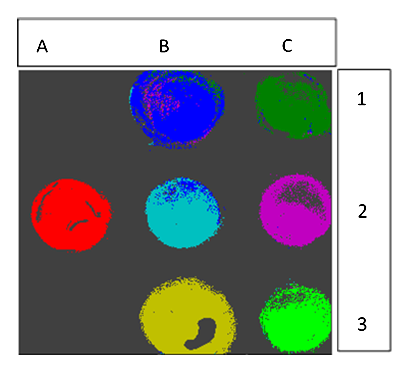
\includegraphics[width=\linewidth]{sample}}
\caption{Badane przetworniki piezoelektryczne.}
\label{fig:sensors}
\end{figure}

Aby dokonać selekcji przetwornika wybrano najprostszy układ geometryczny (patrz: Rys. \ref{fig:sensor_sel_geometry})

\begin{figure}[htbp]
\centering
\fbox{TUTAJ RYSUNEK GEOMETRII CZUJNIKA }%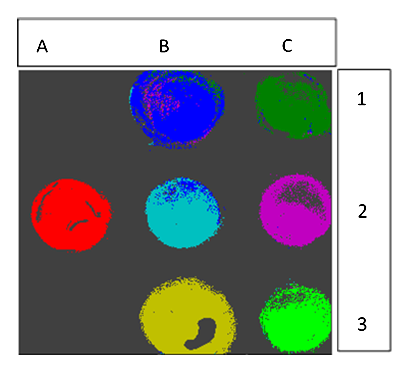
\includegraphics[width=\linewidth]{sample}}
\caption{Konstrukcja pozwalająca na selekcję przetwornika piezoelektrycznego.}
\label{fig:sensor_sel_geometry}
\end{figure}

